\xiti
\begin{xiaotis}

\xiaoti{已知屋椽 $AB$ 和 $AC$ 的长相等,它们的夹角是 $118^\circ$, 计算屋椽与水平线 $BC$ 所成的角的度数。}

\begin{figure}[htbp]
    \centering
    \begin{minipage}[b]{7cm}
        \centering
        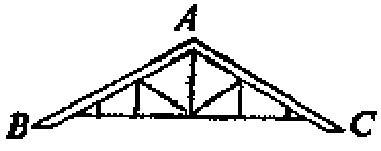
\includegraphics[width=6cm]{../pic/czjh1-ch3-xiti8-01.png}
        \caption*{(第 1 题)}
    \end{minipage}
    \qquad
    \begin{minipage}[b]{7cm}
        \centering
        \begin{tikzpicture}
    \tkzDefPoints{0/0/B,  2/0/C}
    \tkzDefPointBy[rotation=center B angle  50](C)  \tkzGetPoint{a1}
    \tkzDefPointBy[rotation=center C angle -70](B)  \tkzGetPoint{a2}
    \tkzInterLL(B,a1)(C,a2)  \tkzGetPoint{A}
    % \tkzDefTriangle[two angles=50 and 70](B,C)  \tkzGetPoint{A}
    \tkzDefPointBy[rotation=center B angle  130](A)  \tkzGetPoint{D}
    \tkzDefPointBy[rotation=center C angle -110](A)  \tkzGetPoint{E}

    \tkzDrawPolygon(A,B,C)
    \tkzDrawSegments(A,D  D,B  A,E  C,E)
    \tkzLabelPoints[above](A)
    \tkzLabelPoints[below](B,C,D,E)
\end{tikzpicture}


        \caption*{(第 3 题)}
    \end{minipage}
\end{figure}

\xiaoti{已知等腰三角形的一个底角等于顶角的 4 倍,求这个等腰三角形各角的度数。}

\xiaoti{已知 $\triangle ABC$ 的 $\angle ABC = 50^\circ$, $\angle ACB = 70^\circ$。
    延长 $CB$ 至点 $D$,使 $BD = BA$。 延长 $BC$ 至点 $E$, 使 $CE = CA$, 连结 $AD$、$AE$。
    求 $\triangle ADE$ 的各角的度数。
}

\xiaoti{如图的三角测平架中,$AB = AC$,在 $BC$ 的中点 $D$ 挂一个重锤,自然下垂。调整架身,使点 $A$ 恰好在重锤线上。}
\begin{xiaoxiaotis}

    \xxt{求证:$AD \perp BC$;}

    \xxt{这时 $BC$ 处于水平位置,为什么?}

\end{xiaoxiaotis}

\begin{figure}[htbp]
    \centering
    \begin{minipage}[b]{7cm}
        \centering
        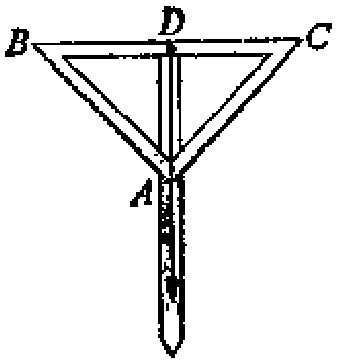
\includegraphics[width=4cm]{../pic/czjh1-ch3-xiti8-04.png}
        \caption*{(第 4 题)}
    \end{minipage}
    \qquad
    \begin{minipage}[b]{7cm}
        \centering
        % 分析题目给的条件,可知: 三角形 ABC 和 三角形 AED 全等,得 AC = AD, 即: 三角形 ACD 是等腰三角形
% 设 CD 的中点 F, 则四边形 ABCF 和 AEDF 关于 AF 轴对称,所以直接定义点的坐标。
\begin{tikzpicture}
    \tkzDefPoints{-1.2/0/C,  1.2/0/D, 0/3/A, -1.8/1.4/B, 1.8/1.4/E} % (0/0/F)
    \tkzDrawPolygon(A,B,C,D,E)
    \tkzLabelPoints[above](A)
    \tkzLabelPoints[right](E)
    \tkzLabelPoints[left](B)
    \tkzLabelPoints[below](C,D)
\end{tikzpicture}

% 也可以绘制一个正五边形(题中没说 AB 与 BC 是否相等,取相等的情况,也是满足题意的)
% \begin{tikzpicture}
%     \tkzDefPoints{0/0/C,  2.5/0/D}
%     \tkzDefRegPolygon[side,sides=5,name=P](C,D)
%     \tkzDrawPolygon(P1,P...,P5)
%     \tkzLabelPoint[right](P3){E}
%     \tkzLabelPoint[above](P4){A}
%     \tkzLabelPoint[left](P5){B}
%     \tkzLabelPoints[below](C,D)
% \end{tikzpicture}


        \caption*{(第 5 题)}
    \end{minipage}
\end{figure}

\xiaoti{已知:如图,$AB = AE$, $BC = ED$, $\angle B = \angle E$。\\
    求证:$\angle C = \angle D$。
}

\xiaoti{求证:等腰三角形底边中点到两腰的距离相等。}

\xiaoti{已知:$AC$ 和 $BD$ 相交于点 $O$, $AB \pingxing DC$, $OA = OB$。\\
    求证: $OC = OD$。
}

\begin{figure}[htbp]
    \centering
    \begin{minipage}[b]{7cm}
        \centering
        \begin{tikzpicture}
    \tkzDefPoints{0/0/A,  4/0/B,  0.8/2.5/D, 3.2/2.5/C}
    \tkzInterLL(A,C)(B,D)  \tkzGetPoint{O}
    \tkzDrawPolygon(A,B,D,C)
    \tkzLabelPoints[above](C,D)
    \tkzLabelPoints[below](A,B)
    \tkzLabelPoints[right=0.5em](O)
\end{tikzpicture}


        \caption*{(第 7 题)}
    \end{minipage}
    \qquad
    \begin{minipage}[b]{7cm}
        \centering
        \begin{tikzpicture}
    \tkzDefPoints{0/0/A,  4/0/B,  1/2.5/D, 3/2.5/C}
    \tkzDefLine[parallel=through C](A,D) \tkzGetPoint{e}
    \tkzInterLL(A,B)(C,e)  \tkzGetPoint{E}
    \tkzDrawPolygon(A,B,C,D)
    \tkzDrawSegment(C,E)
    \tkzLabelPoints[above](C,D)
    \tkzLabelPoints[below](A,B,E)
\end{tikzpicture}


        \caption*{(第 8 题)}
    \end{minipage}
\end{figure}

\xiaoti{已知:如图, $\angle A = \angle B$, $CE \pingxing DA$, $CE$ 交 $AB$ 于 $E$。 \\
    求证: $CE = CB$。
}

\xiaoti{求证:等腰三角形两个底角的平分线的交点到底边的两端距离相等。}

\xiaoti{已知:如图,点 $D$、$E$ 在 $BC$ 上,$\angle BAD = \angle CAE$, $\angle B = \angle C$。 \\
    求证: $AD = AE$。
}

\begin{figure}[htbp]
    \centering
    \begin{minipage}[b]{5cm}
        \centering
        \begin{tikzpicture}
    \tkzDefPoints{0/0/B,  4/0/C,  2/2.5/A}
    \tkzDefPointOnLine[pos=0.3](B,C)  \tkzGetPoint{D}
    \tkzDefPointOnLine[pos=0.3](C,B)  \tkzGetPoint{E}
    \tkzDrawPolygon(A,B,C)
    \tkzDrawSegments(A,D  A,E)
    \tkzLabelPoints[above](A)
    \tkzLabelPoints[below](B,C,D,E)
\end{tikzpicture}


        \caption*{(第 10 题)}
    \end{minipage}
    \qquad
    \begin{minipage}[b]{4.7cm}
        \centering
        \begin{tikzpicture}
    \tkzDefPoints{0/0/B,  4/0/C,  2/2.5/A}
    \tkzDefPointOnLine[pos=0.4](A,B)  \tkzGetPoint{D}
    \tkzDefLine[altitude](B,D,C)  \tkzGetPoint{E}
    \tkzInterLL(E,D)(C,A)  \tkzGetPoint{F}
    \tkzDrawPolygon(A,B,C)
    \tkzDrawSegments(A,F  E,F)
    \tkzMarkRightAngle(C,E,F)
    \tkzLabelPoints[above,xshift=0.5em](A)
    \tkzLabelPoints[below](B,C,E)
    \tkzLabelPoints[left](D,F)
\end{tikzpicture}


        \caption*{(第 11 题)}
    \end{minipage}
    \qquad
    \begin{minipage}[b]{4.3cm}
        \centering
        \begin{tikzpicture}
    \tkzDefPoints{0/0/A,  2.5/0/B}
    \tkzDefPoint(70:4){D}
    \tkzDefShiftPoint[B](50:1.5){C}
    \tkzDrawPolygon(A,B,C,D)
    \tkzLabelPoints[left](A,D)
    \tkzLabelPoints[right](B)
    \tkzLabelPoints[above=0.5em](C)
    %\tkzCalcLength(C,D) \tkzLabelSegment(C,D){\tkzLengthResult}
\end{tikzpicture}


        \caption*{(第 13 题)}
    \end{minipage}
\end{figure}


\xiaoti{已知: $\triangle ABC$ 中, $AB = AC$, $D$ 是 $AB$ 上一点, $DE \perp BC$,
    $E$ 是垂足, $ED$ 的延长线交 $CA$ 的延长线于点 $F$。 \\
    求证: $AD = AF$。
}

\xiaoti{}%
\begin{xiaoxiaotis}%
    \xxt[\xxtsep]{在 $\triangle ABC$ 中, $AB = AC$, $D$ 为 $AC$ 上一点。\\
        求证: $\angle ADB > \angle ABD$。
    }

    \xxt{在 $\triangle ABC$ 中, $AB > AC$, $AD$ 是高。\\
        求证: $\angle BAD > \angle CAD$。
    }

\end{xiaoxiaotis}


\xiaoti{已知:如图,$AD$ 边最大,$BC$ 边最小。\\
    求证: $\angle B > \angle D$。
}


\xiaoti{已知:$\triangle ABC$ 中,$AC > AB$, $D$ 是 $BC$ 上一点。\\
    求证: $AC > AD$。
}

\xiaoti{在 $\triangle ABC$ 中, $AB = AC$, $D$ 是 $BC$ 延长线上一点,
    $E$ 是 $AB$ 上一点, $DE$ 交 $AC$ 于点 $F$。 \\
    求证: $AE < AF$。
}

\end{xiaotis}

